\section{Synthesis of the equivalent transmi,ssion for full pupil illumination}
\label{sec:discussion}

Both the telescope reflectivity and filter transmission display a very
clear radial dependency. While the latter is expected due the
interferometric nature of the filters, the origin of the former is not
yet understood. We can nevertheless build an empirical model assuming
smooth transitions between the measurements, and compute from there a
theoretical "full pupill" transmission by averaging the model over the
illuminated portion of the primary mirror. As is demonstrated in Table
TX, these two steps are necessary to reach sub-percent accuracy in
colors and sub-nm accuracy in central wavelengthes. Last we proceed
with propagating the statistical and systematic errors on the final
transmission curves. The impact of these errors in the interpretation
of broadband photometry is better understood when integrated as errors
on the filter normalisation and central wavelength, which can readily
be translated in errors in colors and color-terms.


\subsection{Radial model of the instrument transmission}
\label{sec:model}

The open transmission of the telescope is modeled as a smooth fonction
of wavelength and incidence angle. The function is developped on a 2D
cubic B-spline basis, with \num{35} wavelength nodes regularly
spaced between \SIrange{350}{1100}{nm}, and 2 nodes in angles between
\SI{1.97}{\degree} and \SI{7.24}{\degree}. The two angles corresponds
to the inner and outer edge of the occultation free primary mirror,
set at \SIrange{55}{203}{mm} in radius assuming a \SI{1600}{mm} focal
length.

For data acquired with a filter in the path, the open transmission
model is multiplied by a model of the interference filter transmission
build as follows:
\begin{equation}
  \label{eq:filtertransmission}
T(\lambda, \theta) = \mathcal T\left(\frac{\lambda}{\sqrt{1 -
    (\sin(\theta) / n_\text{eff})^2}}\right)
\end{equation}
where $n_\text{eff}$ is an effective index for the inserted filter,
and $\mathcal T$ is the sum of a trapezoidal function which captures
the bulk of the shape, and a spline function which capture residual
features, such as leaks. The trapezoidal function is parametrized by 4
wavelengthes marking the beginning and end of its rising and falling
fronts at normal incidence, and the height of its plateau. The spline
function is developped on bspline basis with 70 nodes in wavelength.

Last photometry of the grating zeroth and first orders are adjusted
with the open transmission multiplied by a spline decomposed on
the same basis as the open transmission.

The composite model is fit to the TX dataset, encompassing data at 4
different radii and successive observations without filters and with
all 7 filters and grating. The baseline model has 1324 free
parameters, \num{288} for each of the 3 smooth transmissions,
$6+72$ for each of the $grizy$ filters and $4+72$ for the $u$ band
filters whose blue edge cannot be reliably determined by the data and
which is set arbitrarily to rise between \SI{340}{345}{nm}. Fit
results are shown in Fig.~\ref{fig:lambdathetafitresults}.

\begin{figure*}
  \centering
  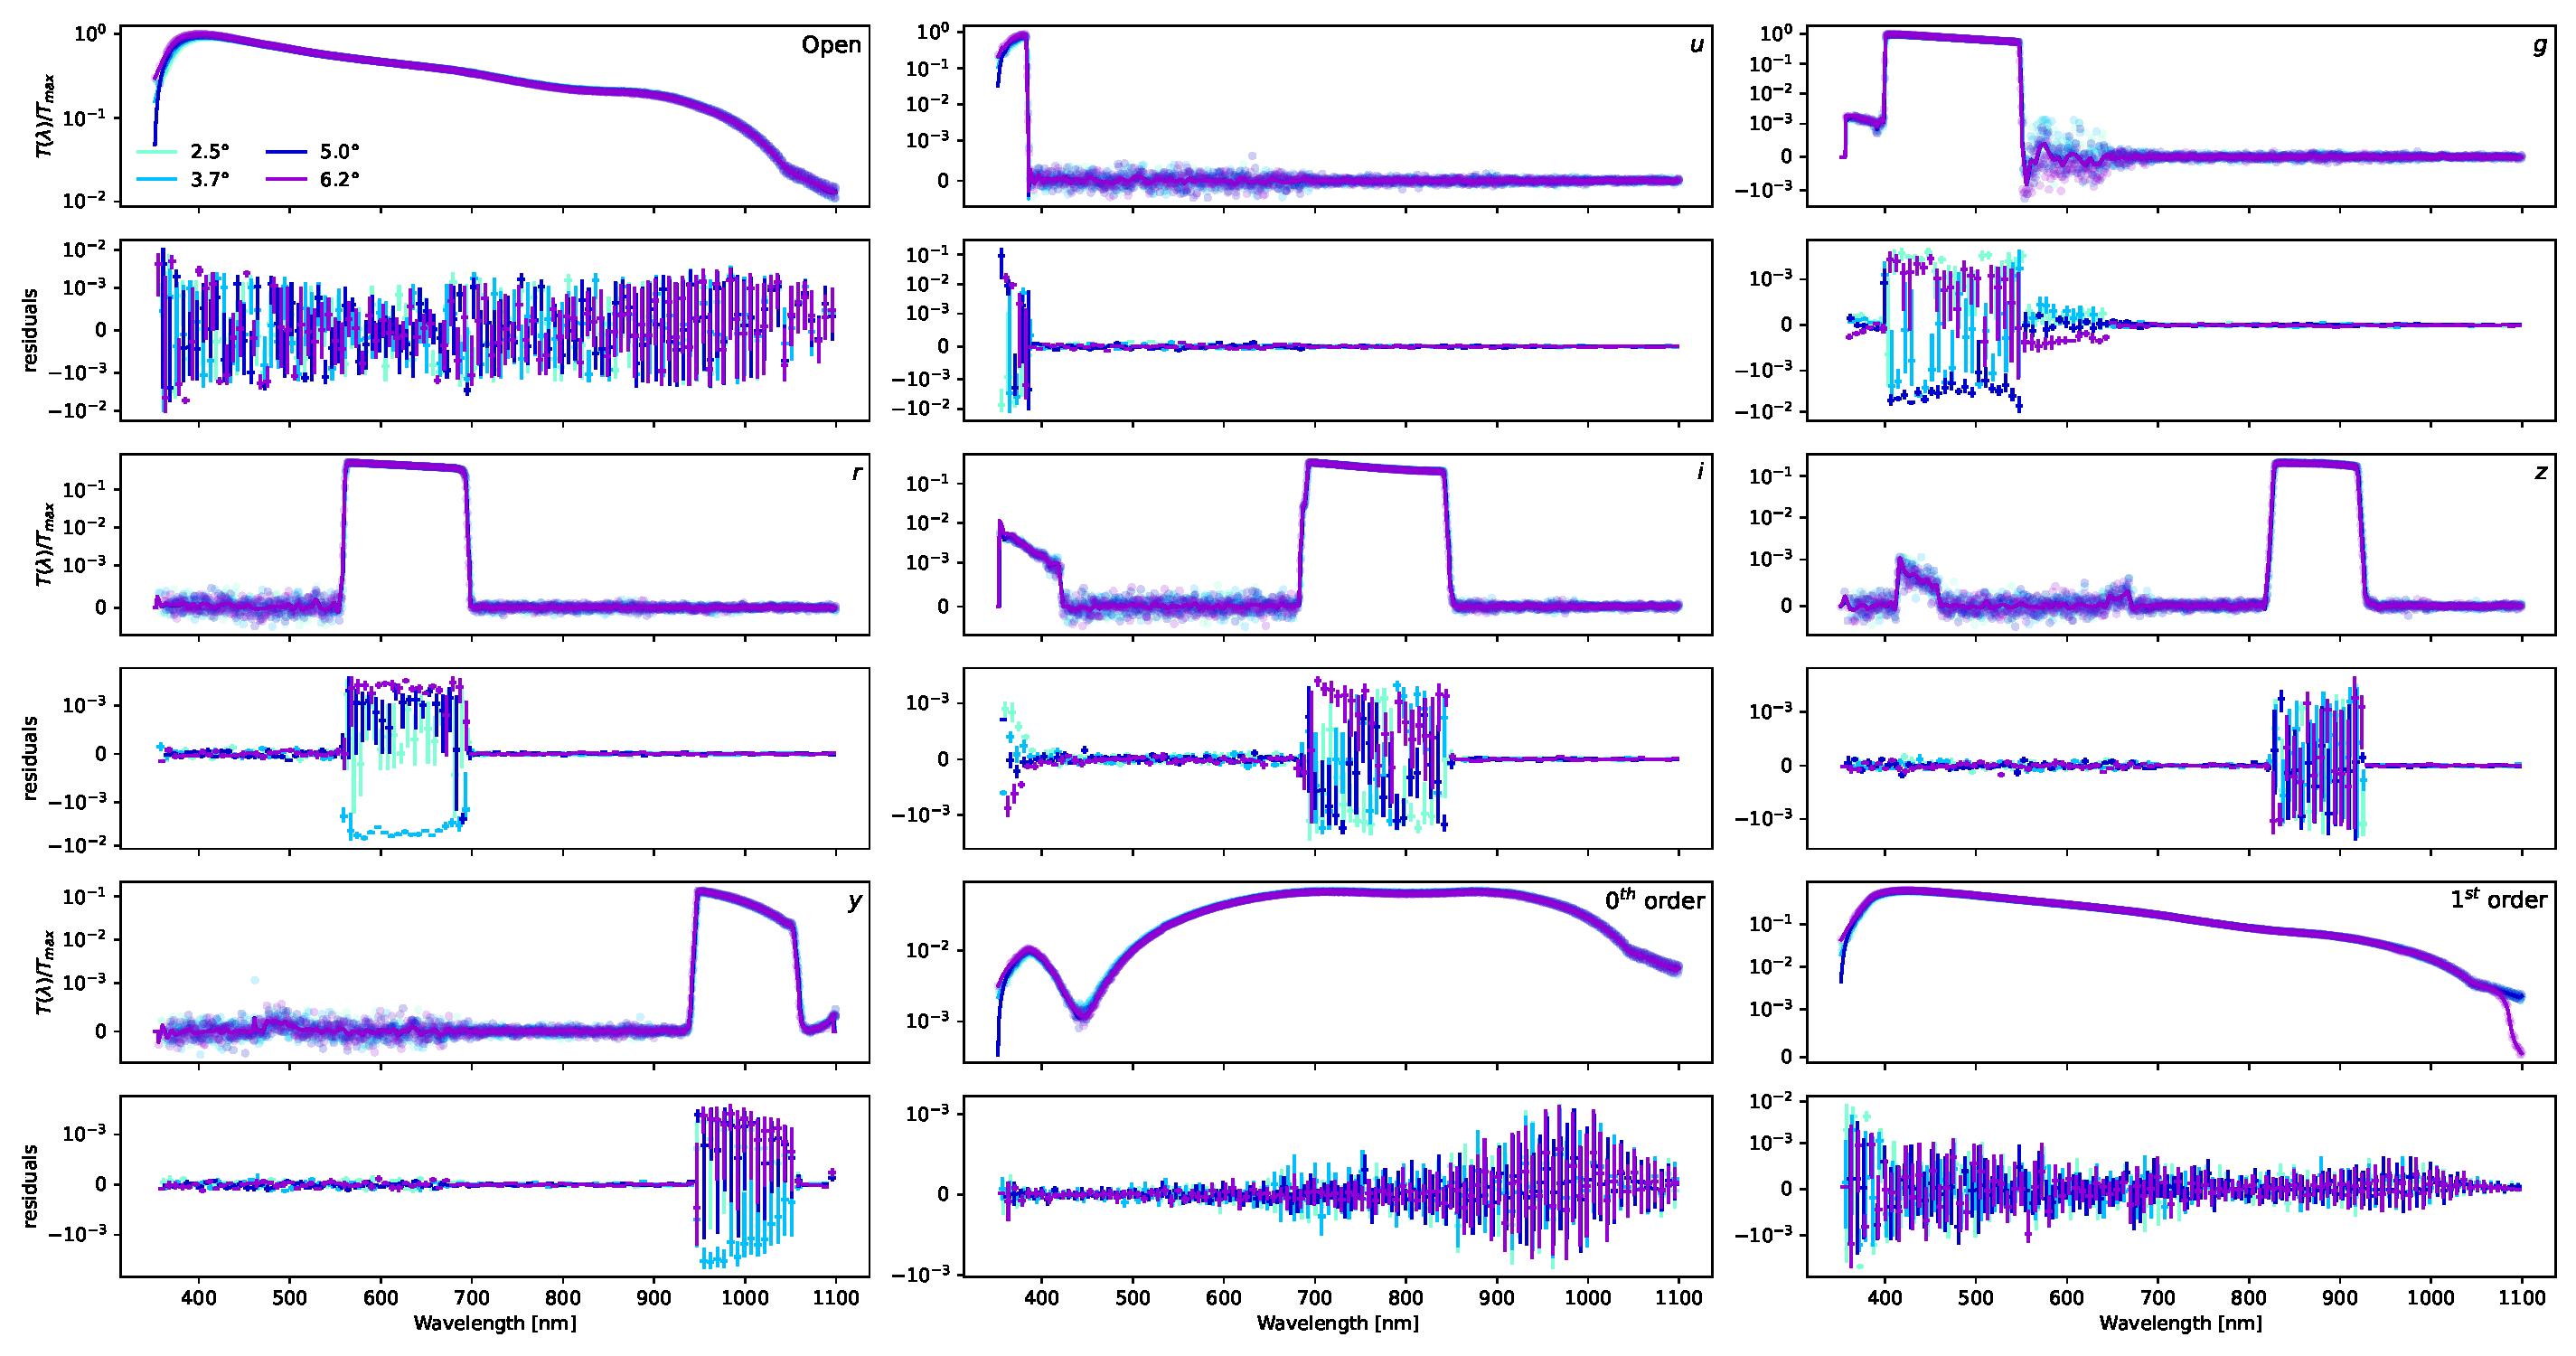
\includegraphics[width=1\linewidth]{./fig/lambdathetafitresults.pdf}
  \caption{Fit results}
  \label{fig:lambdathetafitresults}
\end{figure*}
\MARC{The spline still struggles on the fronts of some filters. Looks
  bad on the plot but I suspect this has little practical
  consequences. I cannot increase infinitly the resolution of the
  spline in the current framework. If to be solved, splines with
  adapted sampling may be the way to go. }

Difference in central wavelength betwen the model and the measurement
is show for all 4 radius in the central panel of
Fig.~\ref{fig:metrics}. The model successfully reproduces the central
wavelength of all filters at better than \SI{0.2}{nm}, which delivers
an improvement by an order of magnitude with respect to a model
neglecting the wavelength shift.

Regarding the assumption that the filter transmission does not depend
on the incidence angle, however, evidences for a departure are visible
from both the fit residuals in Fig.~\ref{fig:lambdathetafitresults} or
from the comparison between model and raw data integrals in the left
panel of Fig.~\ref{fig:metrics}. The discrepancies are nevertheless
contained below the percent level for the core filters $griz$.

We also tested the model against the 4 remaining mirror samples that
are not part of the training dataset. The result of the test is
summarized in Fig.\ref{fig:metrics}.

\begin{figure*}
  \centering
  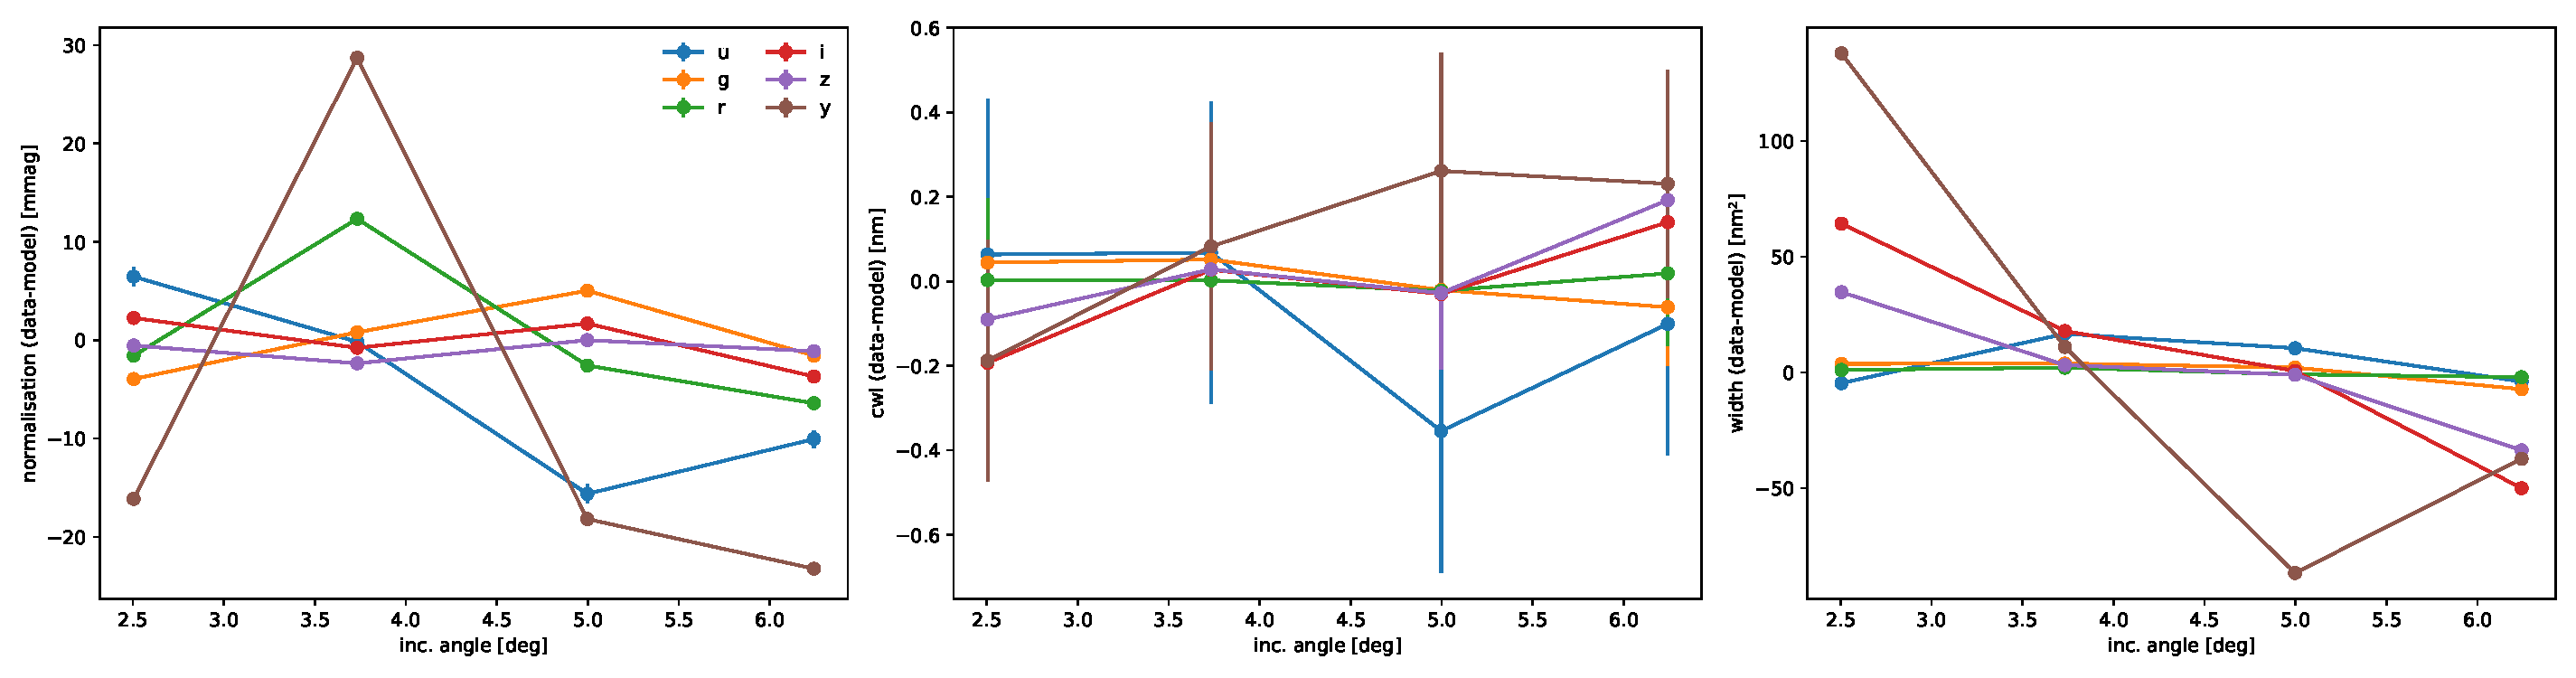
\includegraphics[width=1\linewidth]{fig/metrics.pdf}
  \caption{Discrepancies between model and raw measurements at different mirror locations summarized according to 3 metrics: summarize}
  \label{fig:metrics}
\end{figure*}
\MARC{I am back working on the geometrical model of the telescope and
  precise measurement of the impact parameter}

\subsection{Full pupil synthetic transmission curves}

The full pupil transmission is synthesized by numerically averaging
the above model assuming that the pupil is a perfect annulus with an
inner radius of \SI{55}{mm} and an outer radius of \SI{203}{mm}. A
rectangular quadrature with 100 evenly sampled points in radius as
been used for the averaging. The curve are then normalized using the
CBP response from Sect. TX corrected for the \SI{5}{mm} to \SI{75}{\micro\meter} pinhole
response change determined in Sect. TX. An estimate of the absolute
transmission curve is then computed assuming an effective mirror area
of TX. The resulting transmission curves are shown in
Fig.~\ref{fig:fullpupiltrans}.
\begin{figure}
  \centering
  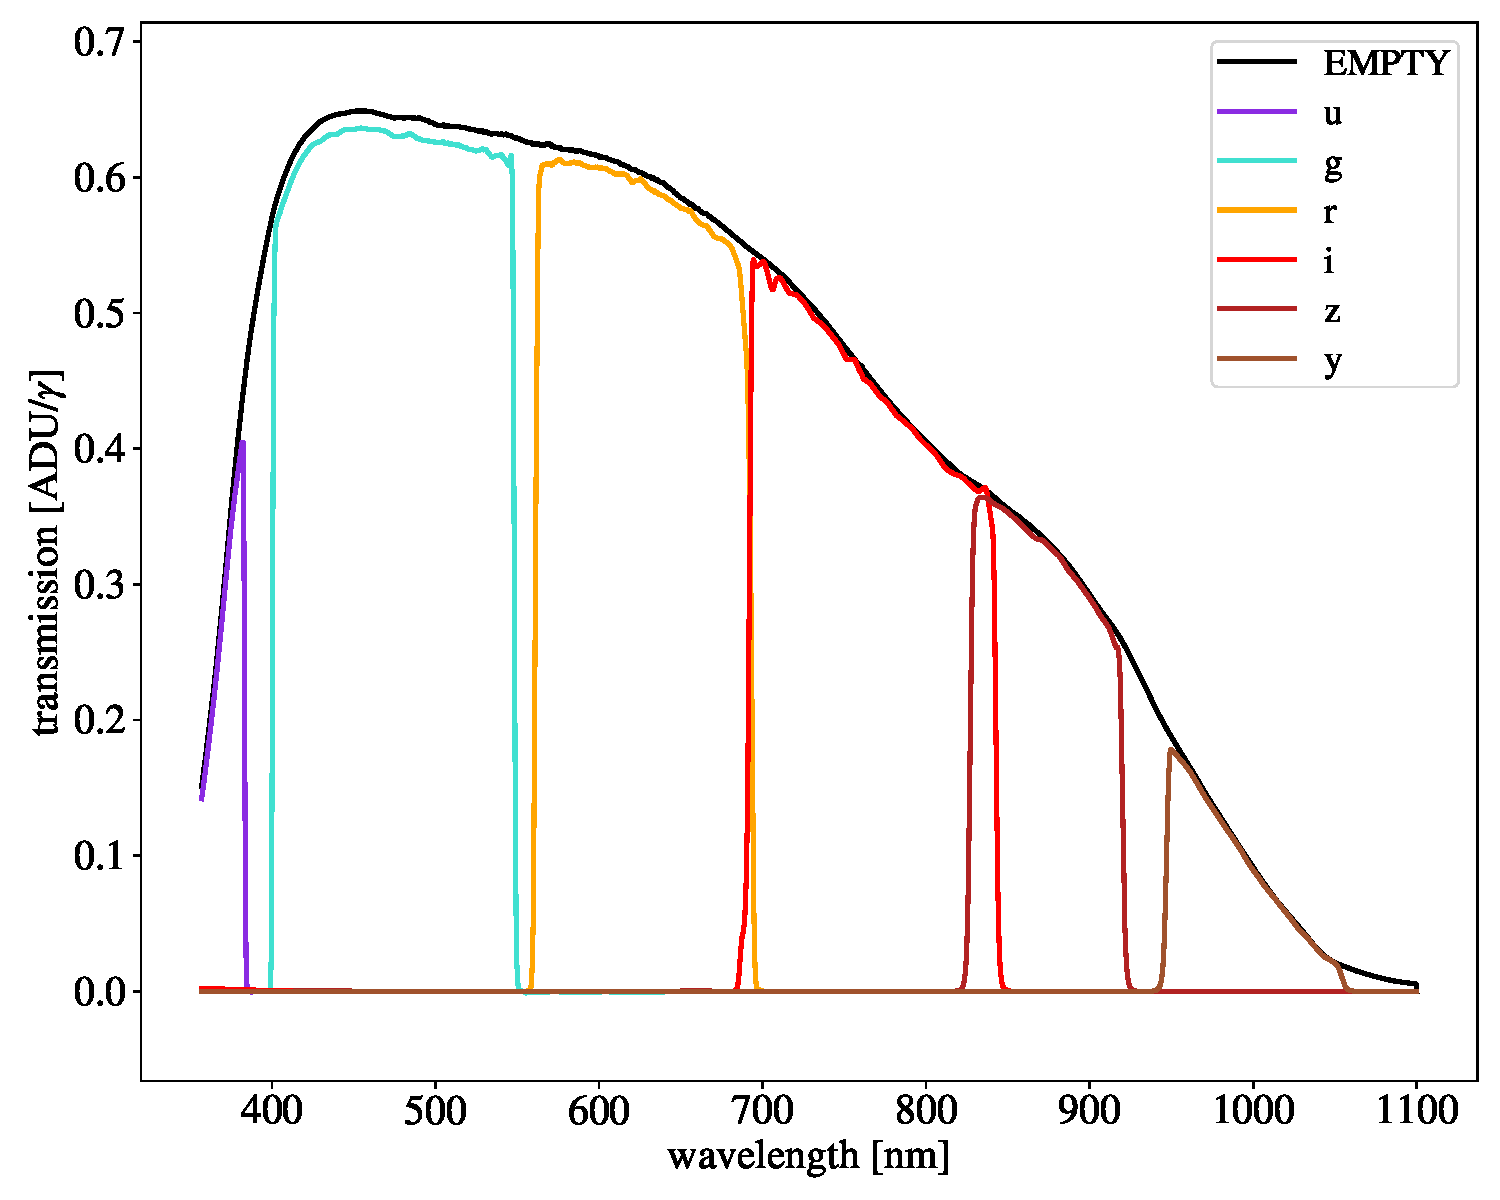
\includegraphics[width=1\linewidth]{fig/fullpupill.pdf}
  \caption{Full-pupill transmission curves for the StarDICE instruments.}
  \label{fig:fullpupiltrans}
\end{figure}


\subsection{Final error budget}
